\documentclass[]{scrartcl}
\title{Vorlesung Analysis II}
\usepackage{amsmath,amssymb,amsfonts}
\usepackage{stmaryrd}
\usepackage{mathtools}
\usepackage{latexsym}
\usepackage{graphicx}
\usepackage{tikz}
\usepackage{xcolor}
\usepackage{soul}
\usepackage{ upgreek }
\usepackage{hyperref}
\usepackage{tipa}
\usepackage[dvipsnames]{xcolor}
\hypersetup{
	colorlinks=true,
	linkcolor=blue,
	filecolor=magenta,      
	urlcolor=cyan,
	pdftitle={Overleaf Example},
	pdfpagemode=FullScreen,
}
\newcommand{\redcircle}[1]{%
	\tikz[baseline=(char.base)]{
		\node[shape=circle, draw=red, text=red, thick, inner sep=1pt] (char) 
		{\textbf{#1}};
	}%
}
\newcommand{\bluecircle}[1]{%
	\tikz[baseline=(char.base)]{
		\node[shape=circle, draw=blue, text=blue, thick, inner sep=1pt] (char) 
		{\textbf{#1}};
	}%
}
\newcommand{\blackcircle}[1]{%
	\tikz[baseline=(char.base)]{
		\node[shape=circle, draw=black, text=black, thick, inner sep=1pt] 
		(char) 
		{\textbf{#1}};
	}%
}
\setul{1pt}{3pt} % Linienhöhe und Abstand zum Text (optional anpassbar)

\setlength{\topmargin}{-.5in} \setlength{\textheight}{9.25in}
\setlength{\oddsidemargin}{0in} \setlength{\textwidth}{6.8in}
\setlength{\parindent}{0pt}

\begin{document}
\textbf{\underline{Teil 1: Differentialrechnung im $\mathbb{R}^n$}}\\
\\
\textbf{\underline{an6: Mittelwertsatz und der Satz von Schwarz}}\\
\\
\textbf{\underline{\underline{Stichworte:} MWS, stetig diff'bar, mehrfache 
partielle Ableitung, Satz von Schwarz}}\\
\\
\textbf{\underline{Literatur:}} \setulcolor{blue}\ul{[Hoff], Kapitel 9.5}\\
\\
\textbf{6.1. \underline{Einleitung:}} Der MWS wird für Skalarfelder 
verallgemeinert.\\
\\
\textbf{6.2. \underline{Erinnerung:}} Hatten der \setulcolor{red}\ul{MWS:} 
Vor.: $a,b \in \mathbb{R}, a\textless b, f:[a,b]\rightarrow \mathbb{R}$ stetig, 
in $]a,b[$ diff'bar.\\
Beh.: $\exists t\in]a,b[: f(b)-f(a)= f'(t)\cdot(b-a).$\\
Dies ist so \underline{nicht} übertragbar auf Abbildungen mit Werten in 
$\mathbb{R}^2$:\\
Betrachte $f:\mathbb{R}\rightarrow\mathbb{R}^2, t\rightarrow\begin{pmatrix}
	\cos t\\\sin t
\end{pmatrix}\in \mathbb{R}^2$ auf $[0,2\pi]$.\\
Aber: $ f(2\pi)-f(0)=0\neq\begin{pmatrix}
	-\sin t\\\cos t
\end{pmatrix}\cdot 2\pi$, da $||\begin{pmatrix}
	-\sin t\\\cos t
\end{pmatrix}||_2=1$ für alle $t\in\mathbb{R}.$\\
\\
\textbf{6.3. \underline{Konvention/Vereinbarung:}} Betrachte also nur 
\underline{$\mathbb{R}^{\textcolor{red}{1}}$}-wertige Funktion (d.h. 
Skalarfelder), die auf $U\subseteq \mathbb{R}$ definiert sind, wo jeder Punkt 
$a\in U$ innerer Punkt von U ist. Für je zwei Punkte $a,b\in U\subseteq 
\mathbb{R}^n$ sei weiter die (Verbindungs-)Strecke $\overline{ab}\subseteq U$, 
wobei \setulcolor{yellow}\ul{$\overline{ab}$}:=$\{a+t(b-a);t\in [0,1]\}$. U 
heißt dann \setulcolor{red}\ul{Konvex (Konvexe Menge).}\\
\begin{figure}[h]
	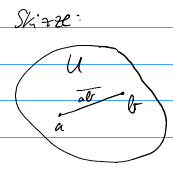
\includegraphics[width=3 cm,height=3cm]{bsp kap 6.3}
\end{figure}\\
\\
\textbf{6.4. \ul{Mittelwertsatz:}}\\
\underline{Vor.:} Sei $\overline{ab}\subseteq U\subseteq \mathbb{R}^n$ wie in 
\setulcolor{blue}\ul{6.3}, $f:U\rightarrow\mathbb{R}$ in allen Punkten von 
$\overline{ab}$ diff'bar.\\
\underline{Beh.:} \setulcolor{green}\ul{$\exists c \in 
\overline{ab}\backslash\{a,b\}$} mit \ul{$f(b)-f(a)=f'(c)\cdot(b-a)$} = 
$\textless f'(c)^T, b-a\textgreater.$\\
\underline{Bew.:} Setze \setulcolor{orange}\ul{$h(t):=f(a+t(b-a))$}, 
$h:[0,1]\rightarrow\mathbb{R}, t\rightarrowtail a +t(b-a)\xrightarrow{f} h(t).$ 
Werde auf h den alten \setulcolor{blue}\ul{MWS An12.13} an:\\
$\exists \xi \in ]0,1[$ mit $h(1)-h(0)=h'(\xi)(1-0) \Rightarrow f(b)-f(a)= 
f'(a+\xi(b-a))(b-a)=f'(c)\cdot(b-a)$\\
mit \setulcolor{orange}\ul{$c:=a+\xi\cdot(b-a)$} 
$\in\overline{ab}\backslash\{a,b\}$.\\
\strut\hfill$\square$\\
\textbf{6.5. \underline{Dies liefert folgende Möglichkeit zur 
Fehlerabschätzung:}}\\
Sei $b=a+\begin{pmatrix}
	\triangle\alpha_1\\\triangle\alpha_2\\\vdots\\\triangle\alpha_n
\end{pmatrix}\in\mathbb{R}^n.$\\
Dann gilt: 
$|f(b)-f(a)|=|f'(c)(b-a)|=|\sum_{j=1}^{n}D_jf(c)\triangle\alpha_j|\leq\sum_{j=1}^{n}
S_j|\triangle\alpha_j|,$\\
wenn $|D_jf(c)|\leq S_j$ mit $1\leq j\leq n$ ist.\\
Dies ist u.U. eine grobe Abschätzung für die Abwechslung des WErts f(b) von 
f(a).\\
\\
\textbf{6.6. \underline{Folgerung:}} \underline{Vor.:} Wie im 
\setulcolor{blue}\ul{MWS 6.4.}, aber 
$f:U\rightarrow$\setulcolor{green}\ul{$\mathbb{R}^m, \max_{1\leq i\leq 
m}||f'(c)^T||_\infty \leq M\in \mathbb{R}_{\textgreater 0}$ für alle $c \in 
\overline{ab}\backslash\{a,b\}$}.\\
\underline{Beh.:} \ul{$||f(b)-f(a)||_\infty\leq nM\cdot||b-a||_\infty$}.\\
\underline{Bew.:} Sei $i\in \{1,...,m\}$ so, dass $||f(b)-f(a)||_\infty = 
|f_i(b)-f_i(a)|.$\\
Mit dem \setulcolor{blue}\ul{MWS 6.4.} folgt: $\exists c \in 
\overline{ab}\backslash\{a,b\}$ mit 
$|f_i(b)-f_i(a)|=|\underbrace{f_i'(c)}_{\in 
\mathbb{R}^{1xm}}\cdot\underbrace{(b-a)}_{\in\mathbb{R}^n}|
\leq ||f_i'(c)^T||_2\cdot||b-a||_2\leq nM\cdot ||b-a||_\infty.$\\
\strut\hfill$\square$\\
Dies Liefert und ein nützliches Kriterium zur Überprüfung der (totalen) 
Differenzierbarkeit:\\
\textbf{6.7. \underline{Satz:}} \underline{Vor.:} $U\subseteq \mathbb{R}^n, 
\forall c \in U:c$ innerer pkt. von 
\setulcolor{green}\ul{$U,f:U\rightarrow\mathbb{R}^m$}, f \ul{partiell diff'bar 
alle partiellen Ableitungen seien in $a\in U$ stetig}.\\
\underline{Beh.:} \ul{f in a diff'bar, f'(a)=$(f_1(a),...,D_nf(a))$}.\\
\underline{Bew.:} Sei $\OE m=1, \OE a=o, \OE n=2, \OE 
||\cdot||=||\cdot||_infty.$ Ferner sei x so klein, dass 
$\overline{\begin{pmatrix}
	0\\\xi_2
\end{pmatrix},\begin{pmatrix}
	\xi_1\\\xi_2
\end{pmatrix}}\subseteq U$.\\
\begin{figure}[h]
	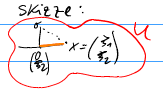
\includegraphics[width=3 cm,height=3cm]{bsp kap 6.7}
\end{figure}\\
Dann gilt: $|f(x)-f(o)-(D_1f(o),D_2f(o))x|\\
=|f\begin{pmatrix}
	\xi_1\\\xi_2
\end{pmatrix}-f(o)-D_1f(o)\xi_1-D_2f(o)\xi_2|\\
\leq |f\begin{pmatrix}
	\xi_1\\\xi_2
\end{pmatrix}-f\begin{pmatrix}
	0\\\xi_2
\end{pmatrix}-D_1f(o)\xi_1|+|\underbrace{f\begin{pmatrix}
	0\\\xi_2
\end{pmatrix}-f(o)-D_2f(o)\xi_2}_{=o(|\xi_2|)\text{,  da die partielleAbl. 
(entlang}\xi \text{)ex.}}|\\
\leq |\underbrace{D_1f\begin{pmatrix}
	z_1\\\xi_2
\end{pmatrix}-D_1f(o)}_{\rightarrow0\text{für} 0\textless z_1\textless 
\xi_1\rightarrow0}|\cdot |\xi_1|+\underbrace{o(|\xi_2|)}_{=o(||x||_\infty), 
\text{da} x\rightarrow o \text{betr. wird}}=o(||x||_\infty).$\\
\strut\hfill$\square$\\
\textbf{6.8. \underline{Def.:}} Wir nennen eine Funktion wie \ul{in 6.7.}. 
\setulcolor{red}\ul{stetig diff'bar}, d.h. wenn sie (partiell) diff'bar ist und 
so, dass alle partiellen Ableitungen stetig sind. Ohne Stetigkeit der partillen 
Ableitungen kann \ul{6.7.} nicht stimmen, vgl. \ul{4.16.}\redcircle{Ü}\\
\\
\textbf{6.9.} Wir untersuchen nun auch höheree Ableitungen. Dazu sei die 
Generalvoraussetzung.\\
Sei $f:U\rightarrow\mathbb{R}^m, a\in U,$ weiter sei\\
\setulcolor{yellow}\ul{$U\subset \mathbb{R}^m$}: 
$\Leftrightarrow$\setulcolor{red} \ul{$U\subseteq\mathbb{R}^n$} und 
\ul{$\forall c\in U:$ c innerer Punkt von U}, d.h. 
\ul{$U\subseteq\mathbb{R}^n$} und \ul{$\forall c \in U \exists \epsilon 
\textgreater0: U_c^\epsilon\subseteq U$}.\\
Diese Bedingung kommt häufig vor. Wir sagen dann, U ist eine \ul{offfene 
Teilmenge von $\mathbb{R}^n$} (als Verallg. von "offene IV").\\
\\
\textbf{6.10 \underline{Beobachtung:}} Falls f in a diff'bar, so haben wir 
$f':U\rightarrow Hom(\mathbb{R}^n,\mathbb{R}^m)\overset{\uppsi}{a}\rightarrow 
f'(\overset{\uppsi}{a})$\\
Falls f' in a diff'bar, so haben wir\\
$f'':U\rightarrow Hom(\mathbb{R}^n,Hom(\mathbb{R}^n,\mathbb{R}^m))\\
\overset{\uppsi}{a}\rightarrowtail A^\uppsi =: f''$ (zweite Ableitung, 
eindeutig), d.h.: $f'(x)=f'(a)+A\cdot(x-a)+o(||x-a||).$\\
Für $h,k\in\mathbb{R}^n$ ist also $Ah \in Hom(\mathbb{R}^n,\mathbb{R}^m), d.h. 
(Ah)k\in\mathbb{R}^m.$\\
Betr. nun $\tilde{A}:\mathbb{R}^n \times \mathbb{R}^n\rightarrow\mathbb{R}^m 
(h,k)\rightarrowtail (Ah)(k).$\\
Diese Abb. ist bilinear, schreibe daher: $Ahk=\tilde{A}(h,k).$\\
\\
\textbf{6.11.} Ableitungen beziehen sich stets auf die Komponentenfunktion 
$f_1,...,f_m$, vgl. \setulcolor{blue} \ul{4.13.}\\
Wir beschränken uns \OE auf \underline{m=1} und betrachten mehrfache 
\underline{partielle Ableitungen}:\\
\underline{Vor.:} Sei $f: U\rightarrow\mathbb{R}, U\subset \mathbb{R}^n, D_if$ 
existiere auf $U, D_if:U\rightarrow \mathbb{R}.$\\
Falls $D_if(D_if)=D_jD_if=:\frac{\delta^2f}{\delta 
\xi_j\delta\xi_i}=f_{\xi_j\xi_i}$,\\
und für i=j schreibe $\frac{\delta^2f}{(\delta x_i)^2}=\frac{\delta^2f}{\delta 
x_i^2}=D_i^2f.$\\
\\
\textbf{6.12.} Induktiv erhalten wir beliebige höhere partiellen Ableitungen 
wie folgt:\\
\underline{Def.:} Seien $p_1,...,p_r\in \mathbb{N}, i_1,...,i_r
\in\{1,...,n\}$, setze $p:=p_1+...+p_r.$\\
Dann heißt \setulcolor{yellow}\ul{$D_{i_1}^{p_1}\circ 
D_{i_2}^{p_2}\circ...\circ D_{i_r}^{p_r}f$} eine \setulcolor{red}\ul{partielle 
Ableitung von f der Ordnung p.}\\
\\
\textbf{6.13. \underline{Bsp.:}} Für $\begin{pmatrix}
	x\\y
\end{pmatrix}\in \mathbb{R}^2$ betrachte f$\begin{pmatrix}
	x\\y
\end{pmatrix}=xe^y+yx^2.$\\
Dann: $D_1f\begin{pmatrix}
	x\\y
\end{pmatrix}=e^y+2xy, D_2f\begin{pmatrix}
	x\\y
\end{pmatrix}=xe^yx^2,\\
D_2D_1f\begin{pmatrix}
	x\\y
\end{pmatrix}=e^y+2x, D_1D_2f\begin{pmatrix}
	x\\y
\end{pmatrix}=e^y+2x.$\\
Hier gilt $D_2D_1f\begin{pmatrix}
	x\\y
\end{pmatrix}=D_1D_2f\begin{pmatrix}
	x\\y
\end{pmatrix}.$ Ist das immer so? Antwort:\\
\\
\textbf{6.14. \ul{Satz von Schwarz:}} Geg.: $f:U\rightarrow\mathbb{R}, a \in U 
\subset \mathbb{R}^n.\\$
Vor.: \setulcolor{green} \ul{$D_kf,D_l f$ ex.} auf U, \ul{$D_l D_k f$ ex.} auf 
U, \ul{$D_kD_lf(a)$ ex.} und \ul{$D_kD_lf(a)=D_lD_kf(a)$}.\\
Bew.: Sei $\OE n=2, k=1, l=2, a=0, ||\cdot||=||\cdot||_\infty, 
\epsilon\textgreater 0$ so dass $U_0^\epsilon\subseteq U.$\\
Wähle $h,k\in \mathbb{R}$ mit $0\textless |h|,|k|\textless\epsilon.$\\
\setulcolor{orange}\ul{Doppelter Differenzenquotient:}\\
\ul{F(h,k)}:=$\frac{1}{hk}(f\begin{pmatrix}
	h\\k
\end{pmatrix}-f\begin{pmatrix}
	h\\0
\end{pmatrix}-(f\begin{pmatrix}
	0\\k
\end{pmatrix}-f\begin{pmatrix}
	0\\0
\end{pmatrix}))\in \mathbb{R}^m.$\\
Dann: $hkF(h,k)=g(h)-g(0)=g'(\tau h)h$ mit $0\textless\tau\textless1$ geeignet 
laut \setulcolor{blue}\ul{MWS 6.4}\\
$=(D_1f\begin{pmatrix}
	\tau h\\k
\end{pmatrix}-D_1f\begin{pmatrix}
	\tau h\\0
\end{pmatrix})h=D_2D_1f\begin{pmatrix}
	\tau h \\\sigma k
\end{pmatrix}\xrightarrow{h,k\rightarrow 
0}$\setulcolor{orange}\ul{$D_2D_1f(o)$}, da \ul{$D_2D_1f$ stetig in o}.\\
Somit ex. $\lim\limits_{(h,k)\rightarrow o}$, sowie 
$\lim\limits_{(h,k)\rightarrow o}F(h,k)=$\ul{$D_2D_1f(o)$}.\\
Bei \ul{umgekehrter Reihenfolge} erhält man ebenso analog:\\
$\lim\limits_{(h,k)\rightarrow o}F(h,k)=$\ul{$D_1D_2f(o)$}. Es folgt, da 
Grenzwerte eindeutig sind: $D_2D_1f(o)=D_1D_2f(o).$\\
\strut\hfill$\square$\\
\textbf{6.15. \underline{Bem.:}} Wie im \setulcolor{blue}\ul{Satz 6.7} 
(Kriterium für totale Diff'barkeit) und im \ul{Satz von Schwarz 6.14} zu sehen 
ist, ist die Eigenschaft, dass die partiellen Ableitungen immer noch stetig 
sind, essentiell.\\
\\
\textbf{6.16. \underline{Def.:}}$\bullet$ Sei $p \in \mathbb{N}$.\\
f:$U\rightarrow\mathbb{R}$(oder auch in $\mathbb{R}^n$ möglich), heißt 
\setulcolor{red}\ul{p-mal stetig (partiell) diff'bar}, falls alle partiellen 
Ableitungen der Ordnung p existieren und stetig sind.\\
$\bullet$ Ein 1-,al stetig partiell diff'bar Fkt. heißt auch \ul{stetig 
(partiell) diff'bar}, vgl. \setulcolor{blue}\ul{6.8.}\\
$\bullet$ Für $U\subset\mathbb{R}^n$ setze 
\setulcolor{yellow}\ul{$\ell^p(U,\mathbb{R})=\ell^p(U)$}:= 
$\{f:U\rightarrow\mathbb{R}, f\text{p-mal stetig (partiell) diff'bar}\}$.\\
Weiter sei \ul{$\ell^\circ(U)$}:=$\{f:U\rightarrow\mathbb{R}:f 
\text{stetig}\}$.\\
Ferner setze \ul{$\ell^\infty(U)$}:=$\bigcap_{p\geq 0} \ell^p(U)$, die Menge 
der beliebig oft ("$\infty$ oft") stetig diff'baren Funktionen.\\
Dies sind trivialerweise $\mathbb{R}-VRe,$ und überdies Standardbeispiele für 
\underline{nicht endlichdimensinale} $\mathbb{R}-VRe$.\\
\\
\textbf{6.17.} Aus dem \setulcolor{blue}\ul{Satz 6.7} folgt unmittelbar:\\
\underline{Kor.:} Jeder stetig differnzierbare Fkt. (d.h. 1-mal stetig partiell 
diff'bare Fkt.) ist (total) diff'bar.\\
\\
\textbf{6.18.} Aus dem \ul{Satz von Schwarz 6.14} folgt unmittelbar:\\
\underline{Kor.:} \underline{Vor.:} f in U p-mal stetig (partiell) diff'bar.\\
\underline{Beh.:} Das ergebniss einer p-maligen partiellen Ableitung ist von 
der Reihenfolge unabhängig.\\
\\
\textbf{6.19. \underline{Bsp.:}} Die zweiten (partiellen) Ableitungen von 
$f:\mathbb{R}^3\rightarrow\mathbb{R}\overset{=v}{\begin{pmatrix}
		x\\y\\z
\end{pmatrix}}\rightarrowtail3x^2-\sin(y)+x^3\cos(z)$\\
sind $D_1D_3f(v)=\frac{\delta}{\delta x}(\frac{\delta}{\delta 
z}(3x^2-\sin(y)+x^3 \cos(z)))=\frac{\delta}{\delta x} (-x^2 
\sin(z))=-3x^2\sin(z)$\\
bzw.$D_3D_1f(v)=\frac{\delta}{\delta z}(\frac{\delta}{\delta 
x}(3x^2-\sin(y)+x^3 \cos(z)))=\frac{\delta}{\delta z} (6x+3x^2 
\cos(z))=-3x^2\sin(z)$,\\
sowie $D_2D_3f(v)=0=D_3D_2f(v)$ bzw. $D_1D_2f(v)=0=D_2D_1f(v),$\\
ferner $D_1^2f(v)=\frac{\delta}{\delta z}(-x^3\sin(z))=-x^3\cos(z).$\\
Nach \ul{6.7} ist f dsiff'bar, da die partiellen Ableitungen $D_1f,D_2f,D_3f$ 
stetig sind.



\end{document}